\documentclass{beamer}
\usetheme{chlenski}
\usepackage[utf8]{inputenc}
\usepackage{graphicx}
\usepackage{outlines}

\title{Intro to Microbial Genomics}
\subtitle{BIOL BC3308, Lecture 1}
\author{Philippe Chlenski}
\date{January 17, 2024}

\renewcommand{\c}[1]{\begin{center}#1\end{center}}
\newcommand{\blu}[1]{\textcolor{blue}{\textbf{#1}}}
\newcommand{\red}[1]{\textcolor{red}{\textbf{#1}}}
\newcommand{\yel}[1]{\textcolor{yellow}{\textbf{#1}}}
\newcommand{\gr}[2][.95]{\c{\includegraphics[width=#1\textwidth]{#2}}}

\begin{document}

\begin{frame}[plain]
\titlepage
\end{frame}

\begin{frame}{Outline}
\tableofcontents
\end{frame}

\section{Course information}

\begin{frame}{Schedule}
\begin{table}
\centering
\begin{tabular}{l l}
    1/17  & Introduction + Lab 1\\
    1/24  & Databases, tools, files + Lab 2\\
    1/31  & Alignment + Lab 3\\
    2/07  & Assembly + Lab 4\\
    2/14  & Phylogeny + Lab 5\\
    2/21  & Short read alignment and SNPs + Lab 6\\
    2/28  & Annotation and functional enrichment\\
    3/06  & Midterm\\
    3/20  & Final project overview + journal club\\
    4/03  & Pipeline presentations\\
    4/24  & Final presentations
\end{tabular}
\end{table}
3/13, 3/27, 4/10, and 4/17: Class does not meet
\end{frame}

\begin{frame}{Grade breakdown}
    \begin{outline}
        \1[] Midterm \hfill 100
        \1[] 6 lab reports \hfill 240 
        \1[] Final project \hfill 300 
        \hline
            \2[] Research question \hfill 20 
            \2[] Methodology \hfill 40 
            \2[] Pipeline \hfill 240 
            \hline
                \3[] Report \hfill 60
                \3[] Code \hfill 60 
                \3[] Presentation 1 \hfill 60
                \3[] Presentation 2 \hfill 60
        \1[] Participation \hfill 60
    \end{outline}
\end{frame}

\begin{frame}{Homework policies}
Submit labs by 12:59 PM on the day of class.\\
\bigskip
Two free 3-day extensions, which must be requested at least 24 hours before the submission deadline.\\
\bigskip
Extensions due to illness or extenuating circumstances handled through Barnard.\\
\bigskip
No extensions on final project assignments.
\end{frame}

\begin{frame}{Academic honesty}
Collaboration on labs and homeworks is encouraged.\\
\bigskip
However, you must write up your own homework. No two assignments should ever be identical.\\
\bigskip
Barnard honor code applies.
\end{frame}

\begin{frame}{Class structure}
Approx. 1 hour lecture, 10 minute break, 2 hours lab. Come prepared to discuss readings. \\
\bigskip
Students break out into small groups. I will be available for questions.\\
\bigskip
Both in-class and take-home portions of the lab must be completed! In-class work is worth 10/40 points.
\end{frame}

\section{Motivation and background}

% \begin{frame}{How much DNA do I share with a banana?}
% Hello world
% \end{frame}

\begin{frame}{What is genomics?}
\begin{columns}[t]
\begin{column}{0.5\textwidth}
    \blu{Genetics (1905):} the study of single genes and their effects.
    \fbox{\gr{l1_figs/s3_tree.png}}
    \end{column}
\begin{column}{0.5\textwidth}
    \red{Genomics (1986):} the study of the entirety of an organism's genetic information, e.g., the genome.
    \fbox{\gr{l1_figs/s3_genome.png}}
    \end{column}
\end{columns}
\end{frame}

\begin{frame}{Genomics for evolutionary classifications}
\gr{l1_figs/s4_related.png}
\end{frame}

\begin{frame}{What is bioinformatics?}
\textit{Bioinformatics, n.} The science of \blu{information and information flow in biological systems}, esp. of the use of computational methods in \red{genetics and genomics}. (Oxford English Dictionary)\\
\bigskip
``The \blu{mathematical, statistical and computing methods} that aim to solve biological problems using \red{DNA and amino acid sequences} and related information.'' --Fredj Tekaia
\end{frame}

\section{Fundamentals}

\begin{frame}{Chemical contents of a cell}
\begin{columns}
    \begin{column}{0.4\textwidth}
        \gr{l1_figs/s7_cell.png}
    \end{column}
    \begin{column}{0.6\textwidth}
        \begin{outline}
            \1[] Water
            \1[] Macromolecules:
                \2 DNA: 3.1\%
                \2 RNA: 20.5\%
                \2 Protein: 55.0\%
                \2 Lipid: 9.1\%
            \1[] Small molecules:
                \2 Sugar
                \2 Ions (Na$^+$, Ka$^+$, Ca$^{2+}$, \ldots)
                \2 \ldots
        \end{outline}
    \end{column}
\end{columns}
\end{frame}

\begin{frame}{Genome organization in Prokaryotes}
\begin{columns}
\begin{column}{0.6\textwidth}
    Does not contain nucleus and membrane-bound organelles like Eukaryotes do.\\
    \bigskip
    Simple genome organization (\blu{contains a single circular} double-stranded DNA chromosome, i.e. haploid).\\
    \bigskip
    Genes usually do not have introns and histone proteins.\\
    \bigskip
    Extrachromosomal elements: plasmids.
\end{column}
\begin{column}{0.4\textwidth}
\c{
    \fbox{\gr{l1_figs/s8_prok.png}}\\
    \bigskip
    % \fbox{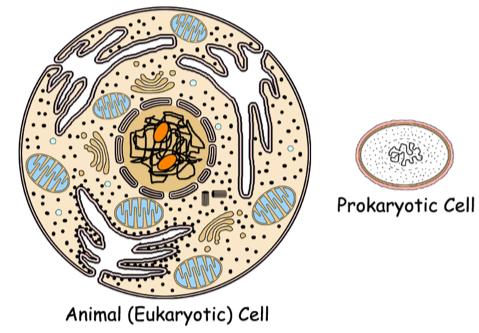
\includegraphics[width=0.5\textwidth]{l1_figs/s8_euk_vs_prok.png}}
    \tiny
    \begin{tabular}{|l|l|}
        \hline
        Bacteria & Genome size\\
        & (Mbp 10^6)\\
        \hline
        \textit{Escherichia coli} & 4.64\\
        \textit{Bacillus subtilis} & 4.20\\
        \textit{Streptococcus pyogenes} & 1.85\\
        \textit{Mycobacterium genitalium} & 0.58\\
        \hline
    \end{tabular}
}
\end{column}\end{columns}
\end{frame}

\begin{frame}{Most genes encode for proteins}
\begin{columns}
    \begin{column}{0.7\textwidth}
        \begin{tabular}{|l|l|l|l|}
        \hline
        & Chromosomes & Bases & Genes\\
        \hline
        Human & 46 & 3B & 20--25K\\
        Dog & 78 & 2.4B & $\sim$ 20K\\
        Corn & 20 & 2.5B & 50-60K\\
        Yeast & 16 & 20M & $\sim$ 7K\\
        \textit{E. coli} & 1 & 4M & $\sim$ 4K\\
        Marbled & ? & 130B & ?\\ 
        lungfish & & & \\
        \hline
        \end{tabular}
    \end{column}
    \begin{column}{0.3\textwidth}
        \small
        \begin{itemize}
            \item Make up the structural components of the cell.
            \item Pass signals
            \item Act as enzymes (catalyze reactions)
            \item Work as molecular motors
            \item \ldots
        \end{itemize}
    \end{column}
\end{columns}
\end{frame}

\begin{frame}{Central dogma of molecular biology}
``Once `information' has passed into protein, it cannot get out again. In more detail, the transfer of information \blu{from nucleic acid to nucleic acid, or from nucleic acid to protein may be possible}, but \red{transfer from protein to protein, or from protein to nucleic acid is impossible}. Information means here the precise determination of sequence, either of bases in the nucleic acid or of amino acid residues in the protein''\\
\c{DNA $\to$ RNA $\to$ Protein}
\small On Protein Synthesis Crick, F.H.C. (1958). Symposia of the Society for Experimental Biology pp. 138--163.
\end{frame}

\begin{frame}{DNA}
\begin{columns}
\begin{column}{0.6\textwidth}
    \begin{outline}
        \1 DNA forms the genetic material of all living organisms
            \2 Can be replicated and passed to descendants
        \1 To computer scientists, DNA is a string made from alphabet $\{\texttt{A, C, G, T}\}$
            \2 e.g. \texttt{ACAGAACGTAGTGCCGTGAGCG}
        \1 Each letter is a nucleotide
        \1 One strand is \blu{reverse- complementary} to the other
    \end{outline}
\end{column}
\begin{column}{0.4\textwidth}
    \gr{l1_figs/s11_dnastrand.png}
\end{column}
\end{columns}
\end{frame}

\begin{frame}{Reverse-complementary DNA sequences}
\gr{l1_figs/s12_rc.png}
\end{frame}

\begin{frame}{Transcription}
\c{
    \gr{l1_figs/s13_transcription.png}\\

    Coding strand:      \hfill \texttt{\blu{5’}-ACGTAGACGTATAGAGCCTAG-\red{3’}}\\
    Template strand:    \hfill \texttt{\red{3’}-TGCATCTGCATATCTCGGATC-\blu{5’}}\\
    mRNA:               \hfill \texttt{\blu{5’}-ACGUAGACGUAUAGAGCCUAG-\red{3’}}
}
\end{frame}

\begin{frame}{Translation}
\begin{columns}
\begin{column}{0.6\textwidth}

\begin{outline}
    \1 The process of making proteins from mRNA.
    \1 A gene uniquely encodes a protein.
    \1 The actual genetic code used by the cell is a triplet.
        \2 Each triplet is called a codon
    \1 The sequence of codons is translated to a sequence of amino acids.
    \1 Start codon: \texttt{AUG}
        \2 Typically Met, but may be others (\texttt{AUG, UUG, GUG, CUG,} etc.)
        \2 Stop codon: \texttt{UGA, UAA, UAG}
\end{outline}

\end{column}
\begin{column}{0.4\textwidth}
    \gr{l1_figs/s14_codons.png}
\end{column}
\end{columns}
\end{frame}

\begin{frame}{Translation example}
Gene: \hfill    \texttt{- \blu{GCT} \red{TGT} \blu{TTA} \red{CGA} \blu{ATT} -}\\
mRNA: \hfill    \texttt{- \blu{GCU} \red{UGU} \blu{UUA} \red{CGA} \blu{AUU} -}\\
Peptide: \hfill \texttt{- \blu{Ala} \red{Cys} \blu{Leu} \red{Arg} \blu{Ile} –}
\end{frame}

\section{Sequencing}

\begin{frame}{Sequencing overview}
Definition: Resolving a nucleotide sequence (whole-genome or less)\\
\bigskip
Many different methods developed:
\begin{outline}
    \1 Maxim-Gilbert (1977)
    \1 Sanger (1977)
    \1 Next generation (high-throughput) methods
\end{outline}
\end{frame}

\begin{frame}{Progression of sequencing technologies}
\gr{l1_figs/s16_sequencing_progression.png}
\end{frame}

\begin{frame}{Sanger sequencing overview}
\gr{l1_figs/s17_sanger.png}
\end{frame}

\begin{frame}{Sanger sequencing method}
\begin{outline}
    \1 Chain-terminating dideoxynucleoside triphosphates (ddXTPs) are employed
        \2 ddATP, ddCTP, ddGTP, ddTTP lack the 3’-OH tail of dXTPs 
    \1 A mixture of dXTPs with small amount of ddXTPs is given to DNA polymerase with DNA template and primer, and fluorescent labeled ddXTPs
    \1 When DNA polymerase encounters a ddXTP, the synthesis cannot proceed 
    \1 Yields copied sequences of different lengths, each terminated by a labeled ddXTP
    \1 Size separation and fluorescent signals reading allows for \blu{base calling}, or identifying which base corresponding to each position in a read
\end{outline}
\end{frame}

\begin{frame}{Next generation sequencing (NGS) overview}
\begin{columns}
\begin{column}{0.7\textwidth}
    \gr{l1_figs/s20_obligatory.png}
\end{column}
\begin{column}{0.3\textwidth}
    \begin{outline}
        \1 Illumina Hiseq/miseq
        \1 PacBio
        \1 Ion Torrent
        \1 SOLiD
        \1 454
        \1 Nanopore
    \end{outline}
\end{column}
\end{columns}
\medskip
Inflection points represent new technologies that have come out (primarily driven by Illumina)
\end{frame}

\begin{frame}{NGS introduction video}
Multimedia slide: Watch video at \url{https://www.youtube.com/watch?v=jFCD8Q6qSTM}
\end{frame}

\section{Lab 1}

\begin{frame}{Lab 1}
Review of Python and basics of working with sequences.\\
\bigskip
Work in groups of 2-3.\\
\bigskip
The lab is to be handed in with the HW at the start of next week
Labs are to be done in class – include partner name when handing in.\\
\bigskip
HWs must be done individually after class.
\end{frame}

\end{document}
